\title{Math 239 Fall 2023 Tutorial Questions Week 9}

\date{2023 Nov. 16/17}
\maketitle

\begin{enumerate}
    \question{Planar or Not}For each of the following graphs, find a planar embedding or an edge subdivision of $K_5$ or $K_{3,3}$. In the latter case, mark the edges in the subdivision of $K_5$ or $K_{3,3}$. 
    \begin{figure}[h]
        \centering
        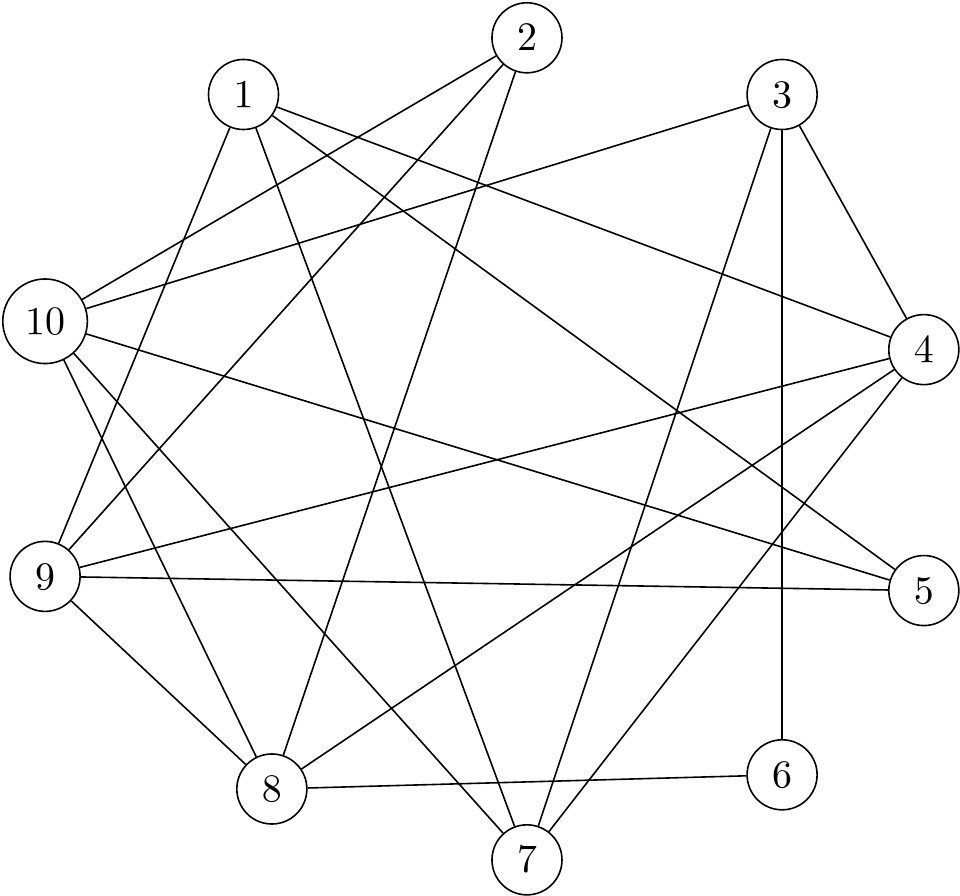
\includegraphics[width=.45\textwidth]{planar.png}\hfill
        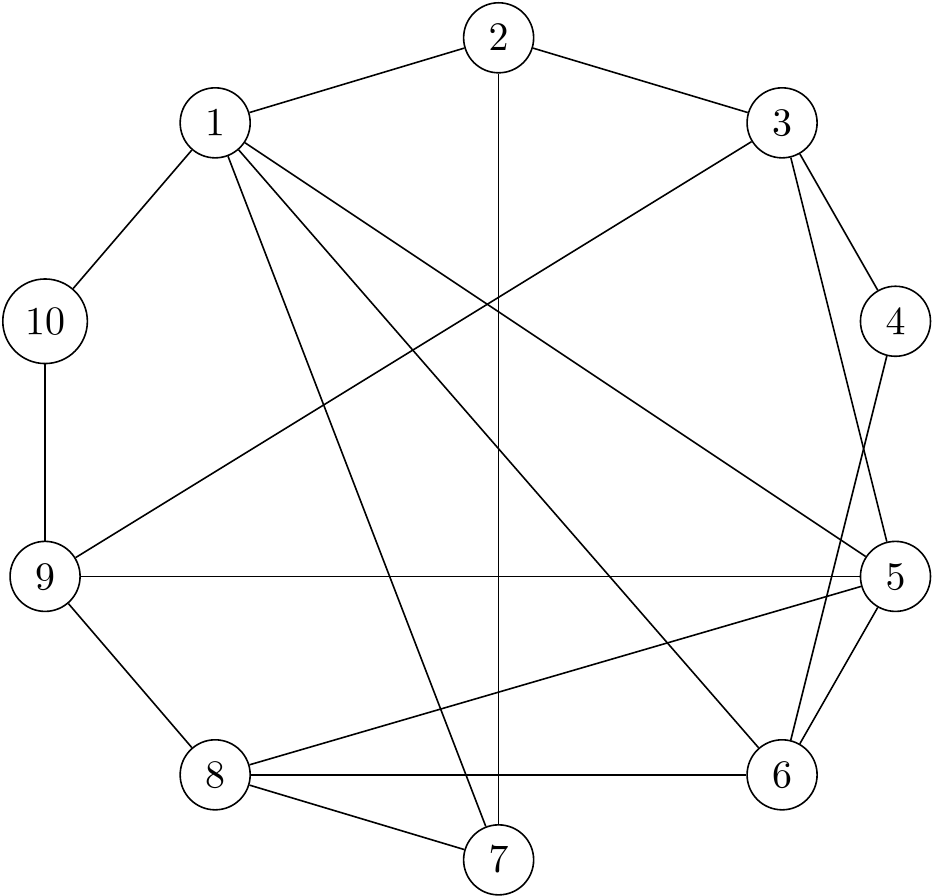
\includegraphics[width=.45\textwidth]{nonplanar.png}
    \end{figure}
    
    \question{Euler's Formula} Suppose $G$ is a connected planar embedding where every vertex has degree $2$ or $5$ and every face has degree $4$.
    \begin{enumerate}
        \item Determine a formula for the number of edges in terms of the number of vertices of degree 5.
        \item Suppose there are exactly $4$ vertices of degree $5$. Determine the number of edges, faces, and vertices of degree $2$. Draw a planar embedding that satisfies these parameters.
    \end{enumerate}

    
    \question{Complete Planar Tripartite Graphs} For positive integers $a \geq b \geq c$ define $K_{a,b,c}$ to be the \textbf{complete tripartite graph} with a tripartition $A,B,C$ (with $|A| = a$ etc.) such that $uv \in E$ iff $u$ and $v$ are in different parts. What are the possible values of $(a,b,c)$ such that $K_{a,b,c}$ is planar? Ignore the trivial cases where any of $a,b,c$ are $0$.

    
    \question{Partitioning Into Planar} Let $n \ge 6$. Prove that the it is not possible to partition the edges of $K_n$ into $\lfloor \frac{n}{6} \rfloor$ planar subgraphs.

    \question{Bonus Question: The Pentagon Problem}
    Let $G$ be a $5$-cycle (a pentagon) with vertices enumerated $1 ,2,3,4,5$ in a circle. Let $c = (c_1 , c_2, c_3, c_4, c_5)$ denote certain numbers we put on vertex $1,2,3,4,5$ respectively (so vertex $3$ has the value $c_3$ on it). We let $c_j \in \mathbb{Z}$, but we requires that $c_1 + c_2 + c_3 + c_4 + c_5 \geq 1$. Now play the following game:
    \begin{itemize}
        \item[] If we have all $c_j>0$ then we have won. Otherwise pick a vertex $j$ with $c_j < 0$. Then ``activate" the vertex to get a new configuration $c'$ with
        \begin{align*}
            c'_i = \begin{cases}
                c_i & \text{if $i$ is not adjacent to $j$},\\
                c_{i} + c_j & \text{if $i$ is adjacent to $j$},\\
                c_{i} - 2c_i & \text{if $i = j$}.
            \end{cases}
        \end{align*}
        Then continue the game from the start with the configuration $c'$.
    \end{itemize}
    Show that we always win, so we always reach a state where $c_j > 0$ for all initial $c$'s.

    This problem is sourced from \textit{The Mathematics of Chip-Firing} by Klivans (problem $2.8.17$). I have no idea how to do it.
\end{enumerate}